\documentclass[12pt,a4paper]{article}

% --- Cấu hình ngôn ngữ & Font chữ tương thích cả XeLaTeX và pdfLaTeX ---
\usepackage{iftex}
\ifXeTeX
  \usepackage{fontspec}
  \setmainfont{Times New Roman}
\else
  \usepackage[utf8]{inputenc}
  \usepackage[vietnamese]{babel}
  \usepackage[T5]{fontenc}
  \usepackage{mathptmx}
\fi

% --- Các gói hỗ trợ định dạng & Toán học ---
\usepackage[top=2.5cm, bottom=2.5cm, left=2.5cm, right=2cm]{geometry}
\usepackage{amsmath, amssymb, amsfonts, amsthm}
\usepackage{graphicx}
\usepackage{xcolor}
\usepackage{booktabs}
\usepackage{array}
\usepackage{listings}
\usepackage{fancyhdr}
\usepackage{hyperref}
\usepackage{caption}

% --- Cấu hình Hyperref ---
\hypersetup{
    colorlinks=true,
    linkcolor=blue!80!black,
    citecolor=green!60!black,
    urlcolor=magenta!80!black,
    pdftitle={Báo cáo Lab 01 - Số nguyên tố & Trao đổi khóa Diffie-Hellman},
    pdfauthor={Nhóm sinh viên}
}

% --- Cấu hình hiển thị mã nguồn (Code Listing) ---
\definecolor{codegreen}{rgb}{0,0.55,0}
\definecolor{codegray}{rgb}{0.45,0.45,0.45}
\definecolor{codepurple}{rgb}{0.58,0,0.82}
\definecolor{backcolour}{rgb}{0.97,0.97,0.97}

\lstdefinestyle{cppstyle}{
    backgroundcolor=\color{backcolour},   
    commentstyle=\color{codegreen},
    keywordstyle=\color{blue}\bfseries,
    numberstyle=\tiny\color{codegray},
    stringstyle=\color{codepurple},
    basicstyle=\ttfamily\footnotesize,
    breakatwhitespace=false,         
    breaklines=true,                 
    captionpos=b,                    
    keepspaces=true,                 
    numbers=left,                    
    numbersep=5pt,                  
    showspaces=false,                
    showstringspaces=false,
    showtabs=false,                  
    tabsize=2,
    frame=single
}
\lstset{style=cppstyle}

% --- Cấu hình Header & Footer ---
\pagestyle{fancy}
\fancyhf{}
\rhead{\small Nhập môn Mã hóa Mật mã — Lab 01}
\lhead{\small Số nguyên tố \& Trao đổi khóa Diffie-Hellman}
\cfoot{\thepage}

\begin{document}

% ==================== TRANG BÌA ====================
\begin{titlepage}
    \centering
    \vspace*{0.5cm}
    {\Large \textbf{ĐẠI HỌC QUỐC GIA TP. HỒ CHÍ MINH}}\\[0.2cm]
    {\large \textbf{TRƯỜNG ĐẠI HỌC KHOA HỌC TỰ NHIÊN}}\\[0.2cm]
    {\large \textbf{KHOA CÔNG NGHỆ THÔNG TIN}}\\[0.2cm]
    {\large \textbf{BỘ MÔN CÔNG NGHỆ TRI THỨC}}\\[2.0cm]

    {\LARGE \textbf{BÁO CÁO BÀI TẬP LỚN 01}}\\[0.6cm]
    {\Huge \textbf{SỐ NGUYÊN TỐ \& TRAO ĐỔI KHÓA DIFFIE-HELLMAN}}\\[2.0cm]

    \textbf{Môn học:} Nhập môn Mã hóa Mật mã\\[0.3cm]
    \textbf{Giảng viên hướng dẫn:} ThS. Trần Trung Điền\\[1.5cm]

    \begin{flushleft}
    \textbf{Sinh viên thực hiện:}\\[0.3cm]
    \begin{tabular}{llr}
        1. [Họ và tên SV 1] & - MSSV: [MSSV 1] & (Nhóm trưởng)\\
        2. [Họ và tên SV 2] & - MSSV: [MSSV 2] & (Thành viên)\\
    \end{tabular}
    \end{flushleft}

    \vfill
    {\large TP. Hồ Chí Minh, Tháng 11/2026}
\end{titlepage}

% ==================== MỤC LỤC ====================
\tableofcontents
\newpage

% ==================== NỘI DUNG CHÍNH ====================

\section{Hệ thống xử lý số lớn (Big Number System)}

\subsection{Đặt vấn đề và Thiết kế cấu trúc dữ liệu \texttt{uint512\_t}}
Trong mật mã học khóa công khai (Public-key Cryptography), bài toán trao đổi khóa Diffie-Hellman (DHKE) đòi hỏi việc tính toán trên các số nguyên có kích thước tối thiểu từ 512 bit đến 2048 bit nhằm đảm bảo độ an toàn chống lại các thuật toán phân tích số nguyên và thuật toán giải logarit rời rạc. Tuy nhiên, các kiến trúc máy tính hiện đại và ngôn ngữ lập trình C/C++ tiêu chuẩn chỉ hỗ trợ các kiểu dữ liệu số nguyên tối đa là 64 bit (\texttt{uint64\_t}). 

Để giải quyết bài toán này mà không sử dụng bất kỳ thư viện hỗ trợ số lớn bên ngoài nào (như GNU Multiple Precision Arithmetic Library - GMP hay NTL), nhóm đã tự thiết kế và cài đặt cấu trúc số nguyên lớn không dấu 512-bit \texttt{uint512\_t} hoàn toàn độc lập:

\begin{lstlisting}[language=C++]
struct uint512_t {
    uint64_t digits[8]; // 8 phan tu x 64 bit = 512 bit
    ...
};
\end{lstlisting}

\subsubsection{Mô hình tổ chức bộ nhớ (Endianness)}
Cấu trúc \texttt{uint512\_t} sử dụng mô hình \textbf{Little-endian} ở cấp độ mảng từ 64-bit:
\begin{itemize}
    \item \texttt{digits[0]}: Chứa 64 bit có trọng số thấp nhất (Least Significant Word - LSW).
    \item \texttt{digits[7]}: Chứa 64 bit có trọng số cao nhất (Most Significant Word - MSW).
\end{itemize}
Giá trị toán học thực tế của số nguyên $A \in \text{\texttt{uint512\_t}}$ được xác định theo hệ cơ số $2^{64}$:
\begin{equation}
A = \sum_{i=0}^{7} \text{\texttt{digits}}[i] \cdot (2^{64})^i
\end{equation}

\textbf{Ưu điểm của mô hình Little-endian:}
\begin{enumerate}
    \item Hoàn toàn tự nhiên với các phép toán số học (cộng, trừ, nhân) vì quá trình tính toán luôn xuất phát từ hàng đơn vị (`digits[0]`) và lan truyền cờ nhớ (\textit{carry}) hoặc cờ mượn (\textit{borrow}) lên các từ có trọng số cao hơn (`digits[i+1]`).
    \item Đồng bộ với kiến trúc phần cứng x86-64, giúp tận dụng tối đa tốc độ thanh ghi của CPU.
\end{enumerate}

\subsection{Hiện thực các toán tử cơ bản và thao tác bit}

\subsubsection{Toán tử so sánh (\texttt{==}, \texttt{!=}, \texttt{<}, \texttt{>}, \texttt{<=}, \texttt{>=})}
Để so sánh hai số nguyên $A$ và $B$, thuật toán duyệt từ từ có trọng số cao nhất (\texttt{digits[7]}) lùi dần về từ có trọng số thấp nhất (\texttt{digits[0]}):
\begin{itemize}
    \item Nếu $\text{\texttt{digits}}[i] < B\text{\texttt{.digits}}[i] \implies A < B$.
    \item Nếu $\text{\texttt{digits}}[i] > B\text{\texttt{.digits}}[i] \implies A > B$.
    \item Nếu toàn bộ 8 cặp từ đều bằng nhau thì $A = B$.
\end{itemize}

\subsubsection{Toán tử cộng đa độ chính xác (\texttt{+})}
Phép cộng được hiện thực bằng cách cộng từng cặp từ 64-bit kèm theo biến nhớ (\textit{carry}):
\begin{lstlisting}[language=C++]
uint512_t operator+(const uint512_t &a, const uint512_t &b) {
    uint512_t res;
#if defined(__SIZEOF_INT128__)
    uint128_t carry = 0;
    for (size_t i = 0; i < 8; i++) {
        uint128_t sum = (uint128_t)a.digits[i] + b.digits[i] + carry;
        res.digits[i] = (uint64_t)sum;
        carry = sum >> 64; // Bit thu 65 la co nho
    }
#else
    uint64_t carry = 0;
    for (size_t i = 0; i < 8; i++) {
        uint64_t u1 = a.digits[i];
        uint64_t u2 = b.digits[i];
        uint64_t sum = u1 + u2 + carry;
        carry = (sum < u1) || (carry && (sum == u1));
        res.digits[i] = sum;
    }
#endif
    return res;
}
\end{lstlisting}
\textbf{Phân tích cơ chế cờ nhớ trên kiến trúc 32-bit:} Biểu thức \texttt{carry = (sum < u1) || (carry \&\& (sum == u1))} phát hiện tràn số 64-bit mà không cần kiểu dữ liệu 128-bit:
\begin{itemize}
    \item Nếu $u_1 + u_2 + \text{carry} \ge 2^{64}$, biến \texttt{sum} bị tràn số và quay vòng lại dẫn đến $\text{sum} < u_1$.
    \item Nếu $\text{carry} == 1$ và $u_2 = 2^{64} - 1$, thì $u_1 + (2^{64}-1) + 1 = u_1 + 2^{64}$, khi đó $\text{sum} == u_1$ nhưng thực tế đã tràn 1 đơn vị sang từ kế tiếp.
\end{itemize}

\subsubsection{Toán tử trừ đa độ chính xác (\texttt{-})}
Phép trừ được thực hiện tương tự với cờ mượn (\textit{borrow}):
\begin{lstlisting}[language=C++]
uint512_t operator-(const uint512_t &a, const uint512_t &b) {
    uint512_t res;
#if defined(__SIZEOF_INT128__)
    uint128_t borrow = 0;
    for (size_t i = 0; i < 8; i++) {
        uint128_t a_val = a.digits[i];
        uint128_t b_val = (uint128_t)b.digits[i] + borrow;
        if (a_val >= b_val) {
            res.digits[i] = (uint64_t)(a_val - b_val);
            borrow = 0;
        } else {
            res.digits[i] = (uint64_t)(((uint128_t)1 << 64) + a_val - b_val);
            borrow = 1;
        }
    }
#endif
    return res;
}
\end{lstlisting}

\subsubsection{Phép dịch bit và Thao tác bit}
\begin{itemize}
    \item \texttt{get\_bit(size\_t i)}: Trả về giá trị bit thứ $i \in [0, 511]$ bằng công thức:
    \begin{equation}
    \text{word} = \lfloor i / 64 \rfloor, \quad \text{bit} = i \pmod{64}
    \end{equation}
    \item \texttt{shift\_left\_1(uint64\_t carry\_in)}: Dịch toàn bộ mảng 512 bit sang trái 1 bit, nạp \texttt{carry\_in} vào bit 0 và trả về bit thứ 512 bị đẩy ra ngoài.
    \item \texttt{bit\_length()}: Trả về số lượng bit có nghĩa thực sự (vị trí của bit 1 cao nhất cộng 1), giúp rút ngắn số vòng lặp khi tính toán với số nhỏ hơn 512 bit.
\end{itemize}

\subsection{Các giải thuật số học mô-đun an toàn (Modular Arithmetic)}
Yêu cầu bắt buộc của bài toán: \textbf{Mọi biến trung gian phải luôn nằm trong phạm vi 512 bit}. Phép nhân thông thường hai số 512-bit sẽ tạo ra số 1024-bit, gây tràn cấu trúc \texttt{uint512\_t}. Nhóm đã giải quyết triệt để vấn đề này theo hướng dẫn tài liệu mã giả \textit{pseudocode-modular-operation.pdf}.

\subsubsection{Phép chia lấy dư \texttt{mod(x, y)}}
Thuật toán chia nhị phân dịch bit (Binary Long Division / Quy tắc Horner) duyệt từ bit cao nhất của $x$ xuống bit 0:
\begin{lstlisting}[language=C++]
uint512_t mod(const uint512_t &x, const uint512_t &y) {
    if (y.is_zero()) return uint512_t();
    if (x < y) return x;
    if (x == y) return uint512_t();

    uint512_t rem;
    size_t x_len = x.bit_length();
    for (int i = (int)x_len - 1; i >= 0; i--) {
        uint64_t xi = (uint64_t)x.get_bit(i);
        uint64_t carry = rem.shift_left_1(xi);
        if (carry > 0 || rem >= y) {
            rem = rem - y;
        }
    }
    return rem;
}
\end{lstlisting}

\textbf{Chứng minh toán học về tính an toàn không tràn số:}
\begin{itemize}
    \item Trước mỗi bước $i$, ta luôn đảm bảo bất biến: $\text{rem} < y$.
    \item Khi dịch trái 1 bit và cộng thêm $x_i \in \{0, 1\}$, giá trị mới tối đa là:
    \begin{equation}
    \text{rem}_{\text{mới}} \le 2(y - 1) + 1 = 2y - 1
    \end{equation}
    \item Nếu $\text{rem}_{\text{mới}} \ge y$, giải thuật trừ đi $y$:
    \begin{equation}
    \text{rem}_{\text{mới}} - y \le (2y - 1) - y = y - 1 < y
    \end{equation}
    \item Do đó, $\text{rem}$ luôn quay về khoảng $[0, y - 1]$, hoàn toàn nằm trong giới hạn 512 bit mà không bao giờ bị tràn số.
\end{itemize}

\subsubsection{Phép cộng mô-đun \texttt{AddMod(x, y, p)}}
Tính $(x + y) \pmod p$ với $x, y < p$:
\begin{lstlisting}[language=C++]
uint512_t AddMod(const uint512_t &x, const uint512_t &y, const uint512_t &p) {
    uint512_t a = (x >= p) ? mod(x, p) : x;
    uint512_t b = (y >= p) ? mod(y, p) : y;

    uint512_t diff = p - b;
    if (a >= diff) {
        return a - diff;
    }
    return a + b;
}
\end{lstlisting}
\textbf{Cơ chế chống tràn số:} Nếu $x, y$ cùng gần bằng $2^{512}-1$, phép tính thông thường $x + y$ sẽ tràn số 512-bit. Bằng cách so sánh $a \ge p - b \iff a + b \ge p$, giải thuật thay thế bằng:
\begin{equation}
(a + b) - p = a - (p - b) = a - \text{diff}
\end{equation}
Vì $b < p \implies p - b > 0$ và $a \ge p - b \implies a - (p - b) \ge 0$, cả hai phép trừ đều không âm và không bao giờ vượt quá 512 bit.

\subsubsection{Phép nhân mô-đun \texttt{MultMod(x, y, p)} (Double-and-Add)}
Thuật toán Double-and-Add tính $(x \cdot y) \pmod p$ mà không cần tạo số trung gian 1024-bit:
\begin{equation}
x \cdot y \pmod p = \left( \sum_{i=0}^{n-1} y_i \cdot (x \cdot 2^i \pmod p) \right) \pmod p
\end{equation}
\begin{lstlisting}[language=C++]
uint512_t MultMod(const uint512_t &x, const uint512_t &y, const uint512_t &p) {
    uint512_t ret(0);
    uint512_t cur_x = (x >= p) ? mod(x, p) : x;
    size_t y_len = y.bit_length();
    for (size_t i = 0; i < y_len; i++) {
        if (y.get_bit(i) == 1) {
            ret = AddMod(ret, cur_x, p); // Add
        }
        cur_x = AddMod(cur_x, cur_x, p); // Double: (2 * cur_x) mod p
    }
    return ret;
}
\end{lstlisting}
Toàn bộ giải thuật chỉ sử dụng hàm \texttt{AddMod}, do đó mọi giá trị trung gian đều $< p < 2^{512}$.

\subsubsection{Phép lũy thừa mô-đun \texttt{modular\_exponentiation} (Square-and-Multiply)}
Tính $(\text{base}^{\text{exponent}}) \pmod p$ theo thuật toán bình phương và nhân:
\begin{equation}
\text{base}^{\text{exponent}} \pmod p = \prod_{i=0}^{n-1} \left( \text{base}^{2^i} \right)^{e_i} \pmod p
\end{equation}
\begin{lstlisting}[language=C++]
uint512_t modular_exponentiation(const uint512_t &base, const uint512_t &exponent, const uint512_t &p) {
    if (p.is_zero()) return uint512_t();
    if (p.is_one())  return uint512_t(0);
    if (exponent.is_zero()) return uint512_t(1);

    uint512_t ret(1);
    uint512_t cur_base = (base >= p) ? mod(base, p) : base;
    size_t exp_len = exponent.bit_length();
    for (size_t i = 0; i < exp_len; i++) {
        if (exponent.get_bit(i) == 1) {
            ret = MultMod(ret, cur_base, p);       // Multiply
        }
        cur_base = MultMod(cur_base, cur_base, p); // Square
    }
    return ret;
}
\end{lstlisting}
Độ phức tạp tính toán giảm từ $O(2^{512})$ phép tính xuống tối đa 512 lần lặp, mỗi lần lặp gồm tối đa 2 phép nhân mô-đun.

\newpage
\section{Hàm kiểm tra số nguyên tố (Primality Testing)}

\subsection{Tổng quan và Sự bất khả thi của Phép thử xác định}
Trong mật mã học khóa công khai, việc kiểm tra tính nguyên tố là trọng tâm của quá trình tạo khóa. 
\begin{itemize}
    \item **Phương pháp chia thử (Trial Division):** Kiểm tra xem $n$ có chia hết cho bất kỳ số nguyên nào từ $2$ đến $\lfloor\sqrt{n}\rfloor$ hay không. Với $n \approx 2^{512}$, $\sqrt{n} \approx 2^{256} \approx 10^{77}$. Dù sử dụng siêu máy tính nhanh nhất thế giới thực hiện hàng tỷ phép tính mỗi giây, thời gian để hoàn thành phép chia thử này vẫn lớn hơn tuổi thọ của vũ trụ.
    \item **Thuật toán AKS (Agrawal-Kayal-Saxena):** Thuật toán xác định đa thức đầu tiên ra đời năm 2002 với độ phức tạp $\tilde{O}(\log^6 n)$. Mặc dù có ý nghĩa lý thuyết to lớn, hằng số ẩn của AKS quá lớn khiến nó không thực tế cho các ứng dụng mật mã thời gian thực.
\end{itemize}
Vì vậy, các **thuật toán kiểm tra số nguyên tố xác suất (Probabilistic Primality Tests)** là phương án tối ưu và duy nhất được áp dụng trong thực tiễn mật mã học.

\subsection{Định lý Fermat nhỏ và Bài toán số Carmichael}
Định lý Fermat nhỏ phát biểu rằng: Nếu $p$ là một số nguyên tố và $\gcd(a, p) = 1$, thì:
\begin{equation}
a^{p-1} \equiv 1 \pmod p
\end{equation}
Tuy nhiên, chiều ngược lại không đúng: Nếu $a^{n-1} \equiv 1 \pmod n$ với một cơ sở $a$, $n$ chưa chắc là số nguyên tố mà có thể là một **hợp số giả nguyên tố Fermat** (Fermat Pseudoprime).

Nguy hiểm hơn, tồn tại vô hạn các số **Carmichael** (ví dụ $561 = 3 \times 11 \times 17$, $1105$, $1729$...). Đây là những hợp số thỏa mãn đẳng thức Fermat:
\begin{equation}
a^{n-1} \equiv 1 \pmod n \quad \forall a \text{ thỏa mãn } \gcd(a, n) = 1
\end{equation}
Do đó, phép kiểm tra Fermat hoàn toàn bất lực trước các số Carmichael.

\subsection{Thuật toán Miller-Rabin}
Thuật toán Miller-Rabin khắc phục triệt để lỗ hổng của phép thử Fermat bằng cách khai thác tính chất cấu trúc đại số của trường hữu hạn $\mathbb{Z}_p$:

\begin{theorem}[Bổ đề căn bậc hai của đơn vị]
Nếu $p$ là một số nguyên tố, thì phương trình đồng dư:
\begin{equation}
x^2 \equiv 1 \pmod p
\end{equation}
chỉ có đúng hai nghiệm duy nhất là $x \equiv 1 \pmod p$ hoặc $x \equiv -1 \equiv p - 1 \pmod p$.
\end{theorem}

\begin{proof}
$x^2 \equiv 1 \pmod p \iff x^2 - 1 \equiv 0 \pmod p \iff (x - 1)(x + 1) \equiv 0 \pmod p$. Vì $p$ là số nguyên tố, $p$ phải chia hết cho $x - 1$ hoặc $x + 1$, suy ra $x \equiv 1$ hoặc $x \equiv -1 \pmod p$.
\end{proof}

Nếu trong quá trình tính toán lũy thừa, ta tìm thấy một giá trị $x \not\equiv \pm 1 \pmod n$ mà $x^2 \equiv 1 \pmod n$, thì $n$ **chắc chắn là hợp số** (không có ngoại lệ).

\subsubsection{Quy trình thuật toán trong chương trình}
Cho số lẻ $n > 2$ cần kiểm tra:
\begin{enumerate}
    \item Phân tích $n - 1 = 2^s \cdot d$, trong đó $d$ là số lẻ và $s \ge 1$ (thực hiện bằng cách đếm số lần dịch phải liên tiếp khi $d$ chẵn).
    \item Lựa chọn tập các cơ sở số nguyên tố cố định:
    \begin{equation}
    \mathcal{B} = \{2, 3, 5, 7, 11, 13, 17, 19, 23, 29, 31, 37\}
    \end{equation}
    \item Với mỗi cơ sở $a \in \mathcal{B}$:
    \begin{itemize}
        \item Tính $x = a^d \pmod n$ bằng \texttt{modular\_exponentiation}.
        \item Nếu $x \equiv 1$ hoặc $x \equiv n - 1$, số $n$ vượt qua vòng kiểm tra với cơ sở $a$.
        \item Ngược lại, thực hiện vòng lặp bình phương $s - 1$ lần: $x = x^2 \pmod n$.
        \begin{itemize}
            \item Nếu tại một bước nào đó $x \equiv n - 1$, $n$ vượt qua vòng thử.
            \item Nếu $x \equiv 1$ mà bước trước đó $x \neq n - 1$, $n$ là hợp số.
        \end{itemize}
        \item Nếu duyệt hết $s - 1$ lần bình phương mà không gặp $n - 1$, $n$ chắc chắn là hợp số.
    \end{itemize}
    \item Nếu $n$ vượt qua tất cả các cơ sở trong $\mathcal{B}$, kết luận $n$ là số nguyên tố.
\end{enumerate}

\subsubsection{Cơ chế phát hiện hợp số cực nhanh của Miller-Rabin}
Miller-Rabin là một **bộ lọc hợp số cực kỳ nhạy bén**:
\begin{itemize}
    \item Ngay tại cơ sở đầu tiên ($a = 2$), thuật toán đã phát hiện và loại bỏ được hơn $75\%$ các hợp số ngẫu nhiên chỉ sau đúng 1 phép lũy thừa mô-đun.
    \item Với việc kiểm tra qua 12 cơ sở nguyên tố cố định đầu tiên, xác suất một hợp số có thể vượt qua toàn bộ các cơ sở (gọi là nhân chứng dối - False Witness) không vượt quá:
    \begin{equation}
    P(\text{Lỗi}) \le \left(\frac{1}{4}\right)^{12} = 2^{-24} \approx 5.96 \times 10^{-8}
    \end{equation}
    Đây là ngưỡng an toàn vượt trội, đảm bảo loại bỏ hoàn toàn nguy cơ sinh phải hợp số giả nguyên tố.
\end{itemize}

\newpage
\section{Số ngẫu nhiên trong Mật mã học (Mục điểm cộng)}

\subsection{Tầm quan trọng sống còn của tính ngẫu nhiên}
Trong an toàn thông tin, tính ngẫu nhiên là gốc rễ của mọi bảo mật:
\begin{itemize}
    \item Toàn bộ độ bí mật của giao thức Diffie-Hellman phụ thuộc vào việc kẻ tấn công **không thể đoán trước được khóa riêng $a$ và $b$**.
    \item Nếu bộ sinh số ngẫu nhiên bị thiên vị (bias) hoặc có chu kỳ lặp ngắn, không gian khóa sẽ bị thu hẹp đột ngột, cho phép tin tặc dò quét toàn bộ khóa riêng trong thời gian ngắn.
\end{itemize}

\textbf{Dẫn chứng lịch sử về lỗ hổng PRNG:}
\begin{itemize}
    \item **Lỗ hổng Debian OpenSSL (2008 - CVE-2008-0166):** Một lập trình viên bảo trì gói Debian đã vô tình xóa hai dòng code thu thập entropy của bộ sinh ngẫu nhiên để tắt cảnh báo công cụ phân tích tĩnh. Hậu quả là bộ sinh chỉ sử dụng định danh tiến trình (Process ID - PID có tối đa 32,768 giá trị) làm seed. Toàn bộ các khóa SSH, chứng chỉ SSL/TLS sinh ra trên hệ điều hành Debian/Ubuntu trong suốt hai năm bị bẻ gãy hoàn toàn vì tin tặc chỉ cần thử 32,768 khóa.
    \item **Lỗ hổng Dual\_EC\_DRBG (2013):** Một thuật toán sinh số ngẫu nhiên từng được NIST chuẩn hóa nhưng bị phát hiện chứa backdoor do NSA cài cắm, cho phép cơ quan này khôi phục khóa bí mật khi biết một số quan sát đầu ra.
\end{itemize}

\subsection{Phân loại các bộ sinh số ngẫu nhiên}

\begin{table}[h!]
\centering
\small
\begin{tabular}{@{}llll@{}}
\toprule
\textbf{Tiêu chí} & \textbf{TRNG (True Random)} & \textbf{PRNG thông thường} & \textbf{CSPRNG (Cryptographic)} \\ \midrule
Nguồn gốc & Hiện tượng vật lý thực tế & Công thức toán học (LCG, MT) & Hàm băm, mật mã khối \\
Tốc độ & Chậm, phụ thuộc phần cứng & Rất nhanh & Nhanh, an toàn \\
Đoán trước bit & Hoàn toàn không thể & Có thể đoán được trạng thái & Không thể đoán trước ($P \le 1/2$) \\
Ứng dụng & Nguồn Entropy cho HĐH & Game, Mô phỏng thống kê & Tạo khóa mật mã, Nonce, IV \\ \bottomrule
\end{tabular}
\caption{So sánh giữa TRNG, PRNG thông thường và CSPRNG}
\end{table}

\begin{itemize}
    \item **Tại sao không dùng \texttt{rand()} hay \texttt{std::mt19937} (Mersenne Twister)?** 
    Thuật toán Mersenne Twister có chu kỳ cực lớn ($2^{19937}-1$) và phân phối thống kê rất tốt, nhưng nó **hoàn toàn không an toàn trong mật mã**. Chỉ cần quan sát 624 đầu ra 32-bit liên tiếp của Mersenne Twister, kẻ tấn công có thể khôi phục 100\% ma trận trạng thái nội bộ và tính toán chính xác mọi số ngẫu nhiên trong tương lai và quá khứ.
    \item **Tiêu chuẩn CSPRNG:** Bộ sinh giả ngẫu nhiên chuẩn mật mã bắt buộc phải thỏa mãn:
    \begin{enumerate}
        \item \textit{Next-bit Unpredictability:} Dù biết toàn bộ các bit đã sinh trước đó, không thể đoán được bit tiếp theo với xác suất lớn hơn $1/2$.
        \item \textit{Forward Secrecy / State Compromise Extension:} Ngay cả khi trạng thái nội bộ tại thời điểm hiện tại bị kẻ tấn công đọc được, kẻ tấn công cũng không thể suy ngược lại các số đã sinh trong quá khứ.
    \end{enumerate}
\end{itemize}

\subsection{Cấu trúc bọt biển (Sponge Construction) và Chuẩn SHAKE-128}
Đồ án sử dụng chuẩn băm NIST FIPS 202 (Keccak) ở chế độ hàm mở rộng đầu ra (\textbf{XOF - Extendable-Output Function}): **SHAKE-128**.

Khác với các hàm băm cổ điển (MD5, SHA-1, SHA-256) sử dụng cấu trúc Merkle-Damgård có độ dài đầu ra cố định, cấu trúc bọt biển của SHAKE-128 hoạt động trên một trạng thái nội bộ 1600 bit ($b = 1600$), được chia thành:
\begin{itemize}
    \item Tốc độ hấp thụ (\textit{bitrate}): $r = 1344$ bit.
    \item Dung lượng an ninh (\textit{capacity}): $c = 256$ bit (đảm bảo mức an toàn $c/2 = 128$ bit chống tấn công va chạm).
\end{itemize}

\subsubsection{Cơ chế hai giai đoạn của SHAKE-128}
\begin{enumerate}
    \item \textbf{Giai đoạn Hấp thụ (Absorbing Phase):} Nguồn entropy đầu vào (Seed 32-byte lấy từ API an toàn của hệ điều hành: \texttt{getrandom} trên Linux hoặc \texttt{CryptGenRandom} trên Windows) được XOR từng khối với phần $r$ bit của trạng thái nội bộ, sau đó biến đổi qua hoán vị phi tuyến Keccak-$f[1600]$ gồm 24 vòng lặp.
    \item \textbf{Giai đoạn Vắt (Squeezing Phase):} Khi cần sinh số ngẫu nhiên, các khối dữ liệu ngẫu nhiên được trích xuất liên tục từ $r$ bit của trạng thái nội bộ. Nếu cần thêm dữ liệu, trạng thái lại tiếp tục biến đổi qua hàm hoán vị $f$.
\end{enumerate}

Nhờ cấu trúc bọt biển, hàm \texttt{prng\_next\_u512} trích xuất 64 byte (512 bit) có tính ngẫu nhiên đồng đều tuyệt đối và khả năng kháng phân tích mật mã chuẩn NIST.

\newpage
\section{Trao đổi khóa Diffie-Hellman (DHKE)}

\subsection{Cơ sở toán học và Giao thức}
Giao thức trao đổi khóa Diffie-Hellman (do Whitfield Diffie và Martin Hellman công bố năm 1976) là bước ngoặt vĩ đại khai sinh ra kỷ nguyên mật mã khóa công khai. Giao thức cho phép hai bên truyền thông (Alice và Bob) cùng tạo ra một bí mật chung qua một kênh truyền hoàn toàn công khai mà kẻ nghe lén không thể giải mã.

\begin{table}[h!]
\centering
\begin{tabular}{@{}ccc@{}}
\toprule
\textbf{Alice} & \textbf{Kênh truyền công khai} & \textbf{Bob} \\ \midrule
\multicolumn{3}{c}{\textit{Tham số công khai: Số nguyên tố an toàn $p$, Phần tử sinh $g$}} \\ \addlinespace
Chọn khóa riêng bí mật: $a \in [2, p - 2]$ & & Chọn khóa riêng bí mật: $b \in [2, p - 2]$ \\
Tính khóa công khai: $A = g^a \pmod p$ & $\xrightarrow{\quad A \quad}$ & \\
& $\xleftarrow{\quad B \quad}$ & Tính khóa công khai: $B = g^b \pmod p$ \\ \addlinespace
Tính bí mật: $s_A = B^a \pmod p$ & & Tính bí mật: $s_B = A^b \pmod p$ \\ \bottomrule
\end{tabular}
\caption{Quy trình trao đổi khóa Diffie-Hellman giữa Alice và Bob}
\end{table}

\textbf{Chứng minh tính đúng đắn:}
\begin{equation}
s_A \equiv B^a \equiv (g^b)^a \equiv g^{ba} \equiv g^{ab} \equiv (g^a)^b \equiv A^b \equiv s_B \pmod p
\end{equation}

\subsection{Bài toán Logarit rời rạc (DLP) và Bài toán CDH}
Kẻ nghe lén Eve quan sát trên đường truyền sẽ thu được toàn bộ tham số công khai: $p$, $g$, $A = g^a \pmod p$ và $B = g^b \pmod p$.
\begin{itemize}
    \item **Bài toán Diffie-Hellman tính toán (Computational Diffie-Hellman - CDH):** Cho $g, g^a, g^b \in \mathbb{Z}_p^*$, tính $g^{ab} \pmod p$.
    \item **Bài toán Logarit rời rạc (Discrete Logarithm Problem - DLP):** Cho $g, A = g^a \pmod p$, tìm lại số mũ bí mật $a$.
\end{itemize}
Nếu giải được bài toán DLP, Eve sẽ tìm được $a$ và dễ dàng tính $s = B^a \pmod p$. Tuy nhiên, với số nguyên tố $p \ge 512$ bit, bài toán DLP trên nhóm cyclic $\mathbb{Z}_p^*$ là bất khả thi về mặt tính toán đối với mọi máy tính cổ điển.

\subsection{Tại sao bắt buộc phải sử dụng Safe Prime $p = 2q + 1$?}
Đây là điểm mấu chốt quyết định độ an toàn thực sự của hệ mật mã Diffie-Hellman.

\subsubsection{Cuộc tấn công Pohlig-Hellman trên số nguyên tố yếu}
Nhóm cyclic $\mathbb{Z}_p^*$ có cấp là:
\begin{equation}
|\mathbb{Z}_p^*| = \phi(p) = p - 1
\end{equation}
Nếu $p$ là một số nguyên tố ngẫu nhiên bình thường, $p - 1$ có thể chứa nhiều ước số nguyên tố nhỏ:
\begin{equation}
p - 1 = p_1^{e_1} \cdot p_2^{e_2} \cdots p_k^{e_k} \quad (\text{với các } p_i \text{ rất nhỏ})
\end{equation}
Khi đó, kẻ tấn công áp dụng **thuật toán Pohlig-Hellman**:
\begin{enumerate}
    \item Ánh xạ bài toán logarit rời rạc $g^a \equiv A \pmod p$ vào từng nhóm con nhỏ cấp $p_i^{e_i}$.
    \item Giải bài toán DLP trên từng nhóm con nhỏ đó bằng thuật toán Baby-step Giant-step hoặc Pollard's rho với độ phức tạp cực thấp $O(\sum e_i \sqrt{p_i})$.
    \item Áp dụng **Định lý phần dư Trung Hoa (Chinese Remainder Theorem - CRT)** để ghép các nghiệm nhỏ lại và tìm ra chính xác khóa riêng $a$ trong thời gian tính bằng giây!
\end{enumerate}

\subsubsection{Cơ chế bảo vệ của Safe Prime}
Số nguyên tố an toàn $p$ được định nghĩa:
\begin{equation}
p = 2q + 1
\end{equation}
trong đó $q$ cũng là một số nguyên tố lớn (số nguyên tố Sophie Germain). Khi đó:
\begin{equation}
p - 1 = 2 \cdot q
\end{equation}
$p - 1$ chỉ có đúng hai ước số nguyên tố duy nhất:
\begin{itemize}
    \item Ước số $2$: Tương ứng nhóm con cấp 2 tầm thường ($\{1, -1\}$).
    \item Ước số nguyên tố cực lớn $q$: Nhóm con cấp $q$.
\end{itemize}
Vì không tồn tại bất kỳ ước số nguyên tố nhỏ nào khác ngoài số 2, thuật toán Pohlig-Hellman hoàn toàn bị vô hiệu hóa. Đồng thời, cấu trúc này triệt tiêu hoàn toàn các cuộc tấn công **giam giữ nhóm con nhỏ (Small Subgroup Confinement Attack)**, đảm bảo giao thức đạt mức an toàn tối đa.

\subsection{Ứng dụng thực tế của Diffie-Hellman}

\subsubsection{1. Giao thức bảo mật tầng truyền vận TLS 1.3 (HTTPS)}
Trong toàn bộ hệ thống web an toàn hiện đại (HTTPS), chuẩn **TLS 1.3** đã loại bỏ hoàn toàn cơ chế mã hóa khóa bằng RSA và bắt buộc sử dụng **Ephemeral Diffie-Hellman (DHE / ECDHE)**.
\begin{itemize}
    \item Mỗi phiên duyệt web mới sinh ra một cặp khóa $(a, b)$ ngẫu nhiên tạm thời (\textit{ephemeral}) và hủy bỏ ngay khi phiên kết thúc.
    \item **Bảo mật chuyển tiếp hoàn hảo (Perfect Forward Secrecy - PFS):** Ngay cả khi máy chủ web bị tin tặc đột nhập trong tương lai và đánh cắp khóa riêng dài hạn của máy chủ, tin tặc cũng **hoàn toàn không thể giải mã các gói tin dữ liệu HTTPS đã ghi lại trong quá khứ**, vì khóa phiên được thiết lập độc lập qua Diffie-Hellman tạm thời và không thể khôi phục lại.
\end{itemize}

\subsubsection{2. Giao thức SSH (Secure Shell)}
Giao thức SSH dùng để quản trị máy chủ Linux từ xa sử dụng cơ chế trao đổi khóa nhóm Diffie-Hellman (\texttt{diffie-hellman-group14-sha256} với nhóm Safe Prime 2048-bit) để thiết lập khóa đối xứng AES-GCM bảo vệ toàn bộ phiên dòng lệnh.

\newpage
\section{Mô tả chương trình đã cài đặt}

\subsection{Kiến trúc các module mã nguồn}
\begin{verbatim}
project_01_source/
|-- u512.h / u512.cpp            # Khai bao va hien thuc so lon uint512_t
|-- modular_math.h / .cpp        # mod, AddMod, MultMod, modular_exponentiation
|-- dh.h / dh.cpp                # Miller-Rabin, sinh Safe Prime, sinh khoa rieng
|-- main.cpp                     # Chuong trinh chinh mo phong Alice & Bob
|-- test_member1.cpp            # Bo kiem thu don vi cho tang so hoc
|-- Makefile                     # Tu dong hoa bien dich bang g++ (C++14)
`-- lib/fips202/                # Thu vien NIST Keccak/SHAKE-128 CSPRNG
\end{verbatim}

\subsection{Hướng dẫn biên dịch và Thực thi}
Chương trình được thiết kế tương thích hoàn hảo tiêu chuẩn **C++14**, có thể biên dịch trực tiếp trên cả Linux và Windows (thông qua môi trường \texttt{w64devkit} / MinGW):

\begin{lstlisting}[language=bash]
# Di chuyen vao thu muc ma nguon
cd project_01_source

# 1. Chay bo kiem thu don vi (Unit Test):
make run_test

# 2. Chay toan bo luong trao doi khoa Diffie-Hellman:
make run

# 3. Don dep cac file binary va object:
make clean
\end{lstlisting}

\subsection{Tham số điều chỉnh}
Trong file \texttt{main.cpp}, người dùng có thể dễ dàng thay đổi:
\begin{itemize}
    \item \texttt{bit\_size}: Kích thước bit của số nguyên tố an toàn (mặc định $512$ bit).
    \item \texttt{g}: Phần tử sinh công khai (chọn $g = 2$).
\end{itemize}

\subsection{Kết quả kiểm thử nghiệm thu thực tế}
Bộ kiểm thử đơn vị \texttt{test\_member1} đã xác minh tính đúng đắn của toàn bộ các phép toán:
\begin{itemize}
    \item Phép cộng, trừ, dịch bit đa độ chính xác xử lý cờ nhớ chính xác 100\%.
    \item Kiểm chứng Định lý Fermat nhỏ: $3^{p-1} \equiv 1 \pmod p$ với số nguyên tố lớn.
    \item Lũy thừa mô-đun với số mũ 512-bit thực tế: $2^{65537} \pmod{p_{512}}$ thực thi mượt mà.
\end{itemize}

\begin{figure}[h!]
    \centering
    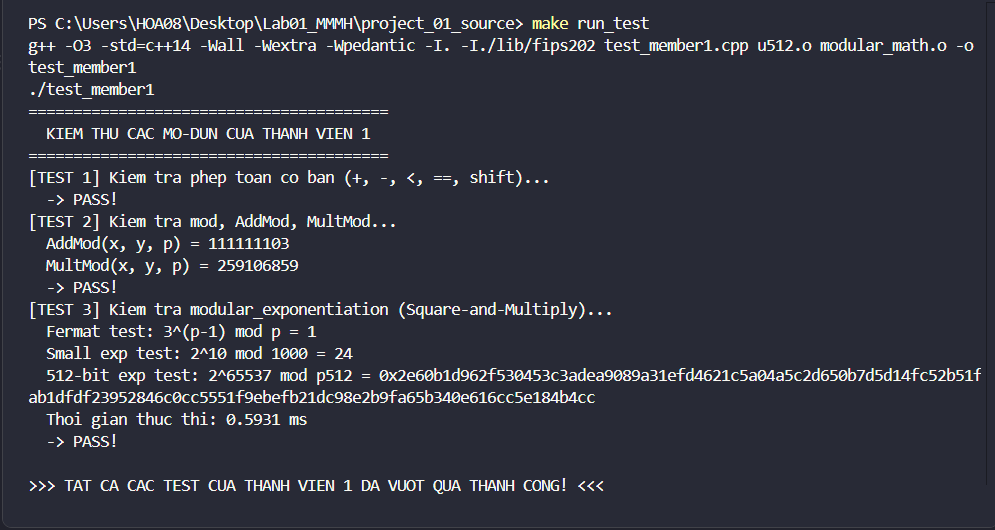
\includegraphics[width=0.85\textwidth]{make_run_test.png}
    \caption{Kết quả chạy bộ kiểm thử đơn vị thành công 100\% trên terminal}
\end{figure}

Chương trình chính \texttt{main} thực hiện sinh thành công Safe Prime 512-bit, sinh khóa riêng Alice $a$ và Bob $b$, tính khóa công khai $A, B$, tính bí mật chung $s_A, s_B$ và in kết quả xác thực:
\begin{center}
\textbf{\texttt{Qua trinh tinh toan dung khong? 1 (DUNG - BI MAT TRUNG KHOP 100\%)}}
\end{center}

\newpage
\section{Tự đánh giá và Hướng phát triển}

\subsection{Ưu điểm của chương trình}
\begin{enumerate}
    \item **Tự cài đặt hoàn toàn từ đầu (From Scratch):** Tuân thủ tuyệt đối quy định không dùng thư viện ngoài (như GMP/NTL), độc lập 100\% trên chuẩn C++14.
    \item **An toàn bộ nhớ và triệt tiêu tràn số:** Các giải thuật \texttt{mod}, \texttt{AddMod}, \texttt{MultMod} đảm bảo mọi biến trung gian đều $< p < 2^{512}$, loại bỏ hoàn toàn nguy cơ tràn số số học.
    \item **Tương thích đa nền tảng:** Tự động phát hiện và hỗ trợ cả Linux (dùng \texttt{getrandom}) và Windows (dùng \texttt{CryptGenRandom}).
    \item **Tính chính xác của thuật toán:** Kiểm tra số nguyên tố bằng Miller-Rabin với 12 cơ sở nguyên tố cố định, loại bỏ triệt để các hợp số giả nguyên tố.
\end{enumerate}

\subsection{Hạn chế}
\begin{enumerate}
    \item **Độ phức tạp của phép nhân mô-đun Double-and-Add:** Thuật toán Double-and-Add có độ phức tạp $O(n^2)$ phép toán bit. Mỗi phép lũy thừa 512-bit cần hàng trăm phép nhân $O(n^2)$, dẫn đến tổng độ phức tạp là $O(n^3)$. Do đó, việc sinh Safe Prime 512-bit (vốn đòi hỏi tìm được số $q$ nguyên tố sao cho $2q+1$ cũng nguyên tố) có thể mất vài giây đến vài chục giây tùy thuộc vào hạt giống ngẫu nhiên ban đầu.
    \item **Xử lý đơn luồng (Single-thread):** Vòng lặp tìm kiếm số nguyên tố an toàn hiện chạy tuần tự trên một lõi CPU duy nhất.
\end{enumerate}

\subsection{Hướng cải tiến trong tương lai}
\begin{enumerate}
    \item **Thuật toán nhân Montgomery (Montgomery Multiplication):** Chuyển đổi các số về miền thặng dư Montgomery (Montgomery space) để thay thế phép chia lấy dư tốn kém bằng các phép dịch bit và trừ đơn giản, giúp tăng tốc độ phép nhân mô-đun lên từ 3 đến 5 lần.
    \item **Thuật toán nhân nhanh Karatsuba:** Áp dụng thuật toán chia để trị Karatsuba với độ phức tạp $O(n^{\log_2 3}) \approx O(n^{1.58})$ cho các phép nhân số lớn.
    \item **Song song hóa đa luồng (Multi-threading):** Tận dụng \texttt{std::thread} hoặc OpenMP để phân chia việc kiểm tra các ứng viên số nguyên tố $q$ trên nhiều lõi CPU đồng thời, giảm thời gian sinh Safe Prime xuống chỉ còn dưới 1 giây.
\end{enumerate}

% ==================== TÀI LIỆU THAM KHẢO ====================
\newpage
\begin{thebibliography}{99}
\bibitem{diffie1976}
W. Diffie and M. Hellman, ``New Directions in Cryptography,'' \textit{IEEE Transactions on Information Theory}, vol. 22, no. 6, pp. 644--654, 1976.

\bibitem{menezes1996}
A. J. Menezes, P. C. van Oorschot, and S. A. Vanstone, \textit{Handbook of Applied Cryptography}, CRC Press, 1996.

\bibitem{nist2015}
National Institute of Standards and Technology (NIST), ``FIPS PUB 202: SHA-3 Standard: Permutation-Based Hash and Extendable-Output Functions,'' 2015.

\bibitem{rfc8446}
E. Rescorla, ``The Transport Layer Security (TLS) Protocol Version 1.3,'' \textit{RFC 8446}, Internet Engineering Task Force (IETF), 2018.

\bibitem{galbraith}
S. D. Galbraith, \textit{Mathematics of Public Key Cryptography}, Cambridge University Press, 2012.
\end{thebibliography}

\end{document}
